%\documentclass[11pt,oneside]{article}

%\usepackage{style-3yp} %this is the .sty file
%\usepackage{rotating}
%\usepackage{multirow}
%\usepackage[normalem]{ulem}
%\usepackage{array}
%\newcolumntype{A}{>{\centering\arraybackslash}m{1cm}}
%\newcolumntype{B}{>{\centering\arraybackslash}m{3cm}}

\lfoot{Lewis Murray} %your name in the footer


%\begin{document}
%\begin{center}
%{\bfseries 3YP - Ammonia Based Storage for Renewable Energy \\ Overall Plant %Financial Analysis}
%\end{center}

\section{Overall Financial Analysis}
\label{LMCostsection}

\subsection{Initial Capital Investment}
The cost estimations for the plant were performed using the 'Total Purchasing Cost Estimate' (TPCE) method \cite{KLM}. This calculates values for the various aspects of the plant's construction by scaling them relative to the purchase price of the major plant components. Table \ref{LMtable:componentPC} shows the purchase prices of the main plant components, and Table \ref{LMtable:TPCE} shows the various scaling factors chosen. In the interest of a conservative estimate, the largest scaling factors were taken from the range of values given.


\begin{table}[h]
\centering
\caption{Purchase Cost of major plant components (data sourced from previous sections)}
\label{LMtable:componentPC}
\begin{tabular}{|c|c|}
\hline
\textbf{Component}  & \textbf{Price (Millions of USD)} \\ \hline
Electrolyser        & 4.37                             \\ \hline
Cryo Separator      & 9.40                             \\ \hline
Reactor             & 15.48                             \\ \hline
Main Turbine        & 75.60                            \\ \hline
HEX Net             & 0.24                             \\ \hline
Wind Farm           & 975.00                           \\ \hline
SOFC/GT system      & 987.91                           \\ \hline
\textbf{TOTAL COST} & \textbf{2068.00}                 \\ \hline
\end{tabular}
\end{table}

\begin{table}[h]
\centering
\caption{Values calculated by TPCE method}
\label{LMtable:TPCE}
\begin{tabular}{|c|c|c|}
\hline
                                                                              \textbf{Expense} & \textbf{\% TPCE}       & \textbf{Cost (Millions of USD)}          \\ \hline
Purchase                                                                      & 100             & 2068.00          \\ \hline
Installation                                                                  & 14          & 289.52           \\ \hline
Instrumentation                                                               & 8          & 165.44           \\ \hline
Piping                                                                        & 20           & 413.60        \\ \hline
Electrics                                                                     & 10           & 206.80           \\ \hline
Building                                                                      & 18          & 372.24           \\ \hline
Yard Improvement                                                              & 5          & 103.40           \\ \hline
Service Facilities                                                            & 20           & 413.60           \\ \hline
Land                                                                          & 2          & 41.36            \\ \hline
\textbf{TOTAL DIRECT COST}                                                    & \textbf{197} & \textbf{4,073.96} \\ \hline
\begin{tabular}[c]{@{}l@{}}Engineering   Supervision\end{tabular}           & 21          & 434.28           \\ \hline
Construction Expenses                                                         & 14          & 289.52           \\ \hline
\textbf{TOTAL INDIRECT COST}                                                  & \textbf{35} & \textbf{723.80}  \\ \hline
\begin{tabular}[c]{@{}l@{}}Contractors   fee\end{tabular}                   & 14          & 289.52           \\ \hline
Contingency                                                                   & 35          & 723.80           \\ \hline
\textbf{FIXED CAPITAL INVESTMENT}                                             & \textbf{281} & \textbf{5,811.08} \\ \hline
Working Capital                                                               & 42          & 868.56           \\ \hline
\textbf{\begin{tabular}[c]{@{}l@{}}TOTAL   CAPITAL INVESTMENT\end{tabular}} & \textbf{323} & \textbf{6,679.64} \\ \hline
\end{tabular}
\end{table}

\subsection{Operating Costs}
The plant operating costs are also calculated using the TPCE method, but with some additional complications. Labour costs are calculated separately, and the values are calculated proportional to the Total Capital Investment instead of the purchase cost. A summary of the operating costs can be seen in Table \ref{LMtable:opcosts}. 
\\

Labour costs were calculated assuming 250 operators are required to be working at the plant at any one time, based on data for a coal power plant of similar power output \cite{Kumar2015}. This was multiplied by 3 so that every hour of the data would be covered over 8 hour shifts. The average salary for a plant operator in the US was found to be \$70,000 \cite{Sokanu}. A total of 750 operators being paid \$70,000 a year results in a cost of \$52.5 million per year. This was multiplied by a safety factor of 10 to account for staff not tied directly to the plant operation, such as administration and security.
\\

The SOFCs must be replaced every 5 years, so this cost will be included in the annual operating costs. This cost is found as the purchase cost for the SOFC system, plus 14\% to account for the installation process, spread equally over 5 years. The other expenses from Table \ref{LMtable:componentPC} are ignored, as these parts are assumed to be covered by the annual maintenance costs. 
\\

In Table \ref{LMtable:opcosts}, 'indirect expenses' accounts for administrative, distributing and marketing expenses, while 'general overhead' accounts for property taxes, personal and property liability insurance, maintenance of plant roads, cafeteria expenses, etc.


\begin{table}[h]
\centering
\caption{Operating costs for the plant}
\label{LMtable:opcosts}
\begin{tabular}{|c|c|c|}
\hline
\textbf{Annual Expense} & \textbf{Calculation}                       & \textbf{Cost (Millions of USD)} \\ \hline
Labour                  & Calculated separately                      & 525.00           \\ \hline
Supervision             & 20\% of Labour Cost                        & 105.00           \\ \hline
Maintenance             & 6\% of TCI                                 & 400.78           \\ \hline
Indirect Expenses       & 3\% of TCI                                 & 200.39           \\ \hline
General Overhead        & 15\% of Labour + Supervision + Maintenance & 690.12           \\ \hline
SOFC Replacement        & 20\% of (Purchase Cost of SOFC + 14\%)     & 225.24           \\ \hline
\textbf{TOTAL}          & \textbf{Sum of all values in this table}   & \textbf{2,146.53} \\ \hline
\end{tabular}
\end{table}



\subsection{Financial Overview}

The levelised cost of electricity per kWh produced is calculated using Equation \ref{LMeq:unitcost}:
\begin{equation}
    \text{Unit Cost of Production} = \frac{\text{Total Operating Cost per Year} - \text{Annual Investment Repayment}}{\text{Total kWh Produced per Year}}
    \label{LMeq:unitcost}
\end{equation}

The plant produces a total of $\text{1.688} \times \text{10}^{\text{10}}$ kWh every year, and the annual investment repayment is calculated using Equation \ref{LMeq:repayment}:
\begin{equation}
    \text{Annual Investment Repayment} = \text{Total Capital Investment}\times\frac{i(1+i)^{n}}{(i+1)^{n} - 1}
    \label{LMeq:repayment}
\end{equation}
Where $i$ is the interest rate and $n$ is the repayment period in years. $i$ is assumed to be 10\%, to account for the high risk involved with investing in new technology, and $n$ is taken to be the currently planned lifetime of the plant, 25 years. This results in an annual repayment of \$735.88 million.
\\

Using Equation \ref{LMeq:unitcost}, the unit cost of production is found to be \$0.17 per kWh. This is much higher than the average sale price of electricity in the US, at \$0.12 per kWh, but much lower than the average sale price in Hawaii, which is \$0.28 per kWh \cite{EIAdata}. This gives a large range of potential sale prices to select, with a very high mark-up being achievable while still being very competitive in Hawaii's energy market. Using an example sale price of \$0.225 per kWh, the forecast is shown in Table \ref{LMtable:profit}.

\begin{table}[h]
\centering
\caption{Annual Revenue, Cost and Profit for the plant}
\label{LMtable:profit}
\begin{tabular}{|c|c|}
\hline
Sale Price per kWh (USD)              & \$0.225     \\ \hline
Total Energy produced per year (kWh)  & $\text{1.688} \times \text{10}^{\text{10}}$ \\ \hline
Annual Revenue (USD)                  & \$3.798 bn. \\ \hline
Annual Expense (USD)                  & \$2.882 bn. \\ \hline
Annual Net Profit (USD)               & \$0.916 bn.\\ \hline
Total Net Profit after 25 years (USD) & \$23.889 bn.\\ \hline
Return on Investment after 25 years   & 342.7\%    \\ \hline
\end{tabular}
\end{table}

\subsection{Conclusion}
It is clearly demonstrated in the cost analysis that the plant is very profitable. However, this is almost entirely due to Hawaii's uniquely expensive energy market. Hawaii's energy is predominantly produced using petroleum, which has to be imported from the US mainland to Hawaii, 2000 miles away in the Pacific Ocean \cite{Solar}. This drives up the price per kWh enormously, and so a very lucrative opportunity is created, whereby electricity generated on the island itself can be sold for much higher than cost price. The cost price shown in Table 4 has been chosen conservatively, and could be set much higher for greater profitability.
\\

It is worth noting that the plant, as it has been modelled in this report, would not be feasible on the US mainland due to the relatively high unit cost per kWh. At \$0.17 per kWh (or \$170 per MWh), it is relatively competitive when compared to some other renewable energy sources, such as solar power and offshore-wind farms (without an ESS), as shown in Figure \ref{LMfig:costcomp}. However, it is still much higher than conventional power generation methods, such as coal-fired power stations. Economies of scale can be capitalised on in order to reduce this cost further, by building an even larger plant to cover a larger demand.
\\
\\
\\
\\
\\
\\


\begin{figure}[t]
    \centering
    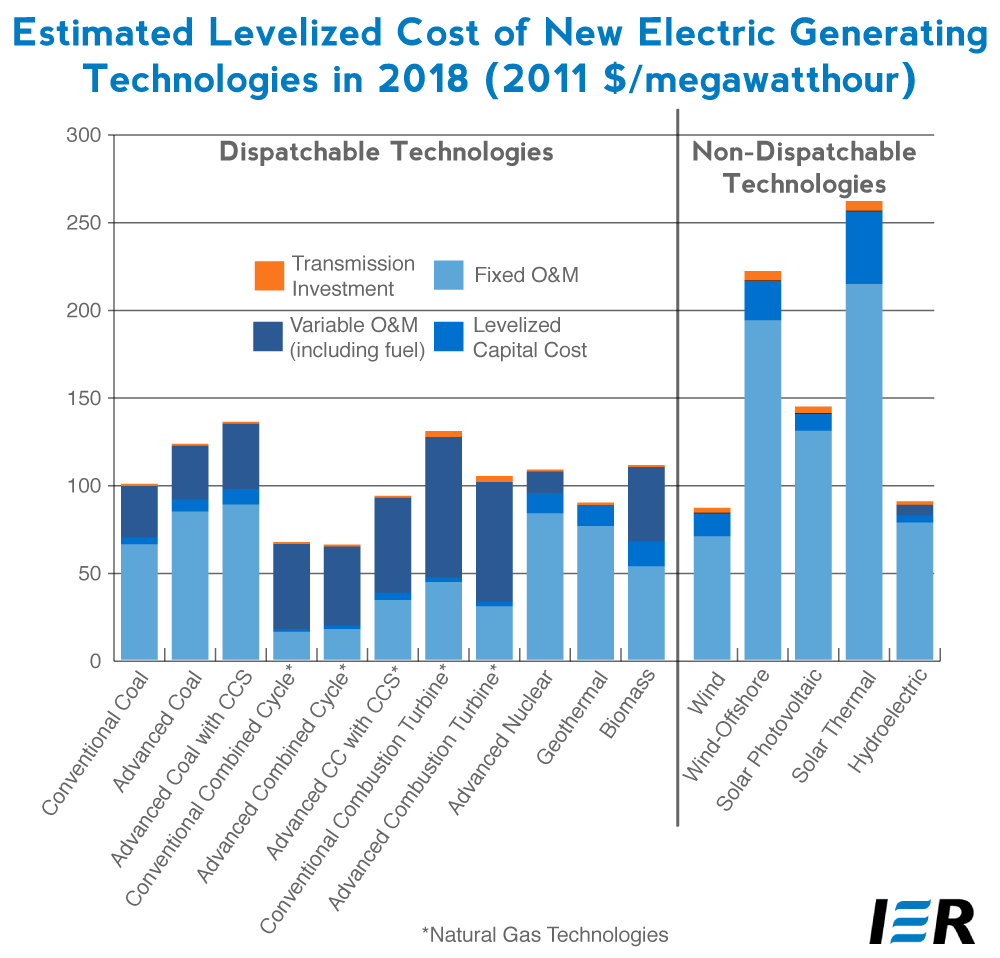
\includegraphics[scale=0.4]{CostComparison.png}
    \caption{Unit cost of production per MWh for various power generation methods \cite{IER}}
    \label{LMfig:costcomp}
\end{figure}

\bibliographystyle{unsrt}
\bibliography{./SOFC/costrefs}





%\end{document}